\newpage
\section{Results}\paragraph{}
The last step in our process is to combine the noise-generated fog with the voxel cone traced shading.

Our clouds can take many shapes and forms. Because of the flexibility of the parameters, we can create many different types of clouds.

The following clouds were rendered on a GTX 965M at 1280x720 resolution. All the clouds rendered at atleast 30 frames per second.

\begin{figure}[h]
\centering
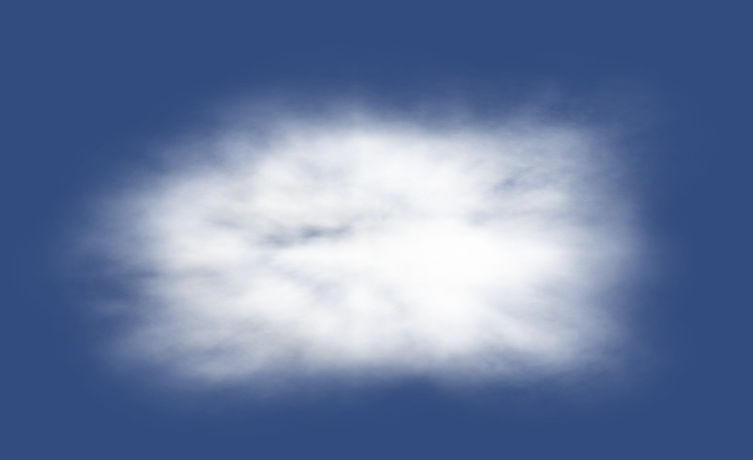
\includegraphics[width=\textwidth]{../res/res1.png}
\caption{view aligned w sun, 10, 1, 16, 0.9, 0.1, 0.1, 1, 0.01, 4, 4, 3, 0.5}
\end{figure}

\begin{figure}[h]
\centering

\includegraphics[width=\textwidth]{../res/res2.png}
\caption{view aligned w sun, 10, 1, 16, 0.9, 0.1, 0.1, 1, 0.021, 1.14, 4, 1.475, 0.5}
\end{figure}

\begin{figure}[h]
\centering

\includegraphics[width=\textwidth]{../res/res3.png}
\caption{view aligned w sun, 10, 1, 22, 0.76, 0.642, 0.0, 1.52, 0.01, 3.03, 4, 1.475, 0.746}
\end{figure}

\begin{figure}[h]
\centering

\includegraphics[width=\textwidth]{../res/res3-1.png}
\caption{view alongside sun, 10, 1, 22, 0.76, 0.642, 0.0, 1.52, 0.01, 3.03, 4, 1.475, 0.746}
\end{figure}

\begin{figure}[h]
\centering
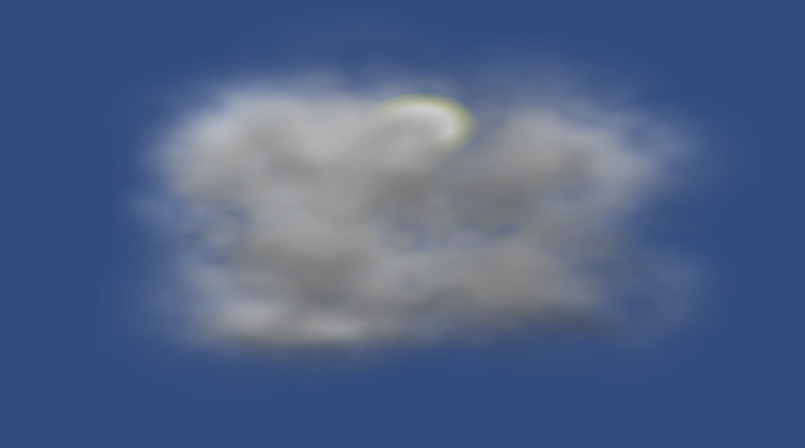
\includegraphics[width=\textwidth]{../res/res3-2.png}
\caption{sun occluded by cloud, 10, 1, 22, 0.76, 0.642, 0.0, 1.52, 0.01, 3.03, 4, 1.475, 0.746}
\end{figure}


\begin{figure}[h]
\centering

\includegraphics[width=\textwidth]{../res/res4.png}
\caption{view aligned w sun, 9.8, 1, 12, 0.74, 0.1, 1.0, 1, 0.01, 5, 4, 0.428, 0.819}
\end{figure}


